\documentclass[border=12pt]{standalone}
\usepackage{amsmath,newtxtext,newtxmath,tikz}
\usetikzlibrary{arrows.meta}
\definecolor{attackred}{HTML}{B71919}
\begin{document}
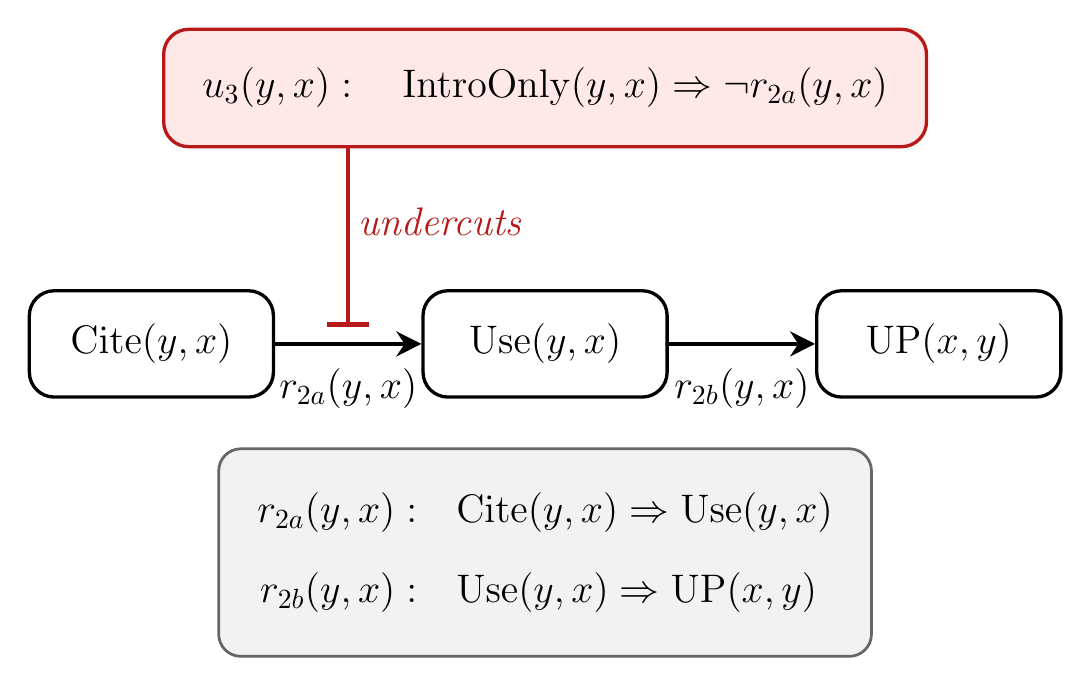
\begin{tikzpicture}[
font=\Large,
claim/.style={draw=black,line width=1.2pt,rounded corners=9pt,minimum width=3.1cm,minimum height=1.35cm,fill=white},
rules/.style={draw=black!60,line width=1pt,rounded corners=8pt,fill=black!5,inner sep=14pt},
flow/.style={-{Stealth[length=9pt,width=9pt]},line width=1.4pt}]

\node[claim] (cite) at (0,0) {$\mathrm{Cite}(y,x)$};
\node[claim] (use) at (5,0) {$\mathrm{Use}(y,x)$};
\node[claim] (up) at (10,0) {$\mathrm{UP}(x,y)$};
\draw[flow] (cite.east) -- node[below=5pt] {$r_{2a}(y,x)$} (use.west);
\draw[flow] (use.east) -- node[below=5pt] {$r_{2b}(y,x)$} (up.west);
\coordinate (attack) at (2.5,0.22);
\node[rules] at (5,-2.65) {$\begin{aligned}
r_{2a}(y,x):\quad &\mathrm{Cite}(y,x)\Rightarrow\mathrm{Use}(y,x)\\[8pt]
r_{2b}(y,x):\quad &\mathrm{Use}(y,x)\Rightarrow\mathrm{UP}(x,y)
\end{aligned}$};

\node[draw=attackred,line width=1.2pt,rounded corners=9pt,fill=red!9,inner sep=14pt] (defeater) at (5,3.25) {$u_3(y,x):\quad \mathrm{IntroOnly}(y,x)\Rightarrow\neg r_{2a}(y,x)$};
\draw[attackred,line width=1.5pt,{Bar[width=15pt]}-] (attack) -- (attack |- defeater.south);
\node[text=attackred,anchor=west,font=\Large\itshape] at (2.5,1.55) {undercuts};
\end{tikzpicture}
\end{document}
